\documentclass[hidelinks,12pt]{article}
\usepackage{graphicx}
\usepackage{hyperref}
\usepackage{xcolor}


\title{Quantum Machine Learning}
\author{Hamza, Ali; Hoda, Bilal}
\date{\today}

\begin{document}

\maketitle

\begin{center}
    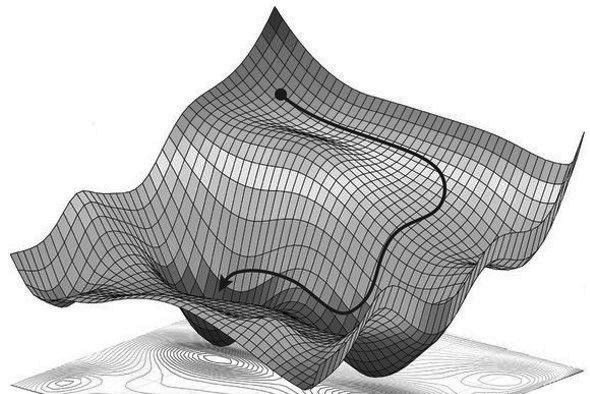
\includegraphics[scale = 0.7]{images/title2.jpg}
\end{center}
\newpage

\tableofcontents
\newpage

\section{Abstract}
\newpage
\section{Introduction}
\subsection{What is Machine Learning?}
\subsection{What is Quantum Machine Learning?}

\newpage
\section{Classical Machine Learning Algorithms}
\subsection{Gradient Descent}
\subsection{Support Vector Machines}

\newpage
\section{Quantum Machine Learning Algoritms}
\subsection{Quantum Gradient Descent}
\subsection{Support Vector Machines via Grover's Algorithm}
\newpage
\section{Quantum Neural Networks}
\newpage
\section{Reflection}
\subsection{Advantages of Quantum Machine Learning}
\subsection{Current Limitations}
\subsection{Future Proespects}
\newpage
\section{Bibliography}




\end{document}
